\chapter{Evaluation}
\label{chap:evaluation}

\glsreset{mae}
\glsreset{mse}
\glsreset{rmse}
\glsreset{r2}
% \glsresetall

This chapter illustrates the evaluation of our generalization strategy by comparing the model variants proposed in Section \ref{sec:model-variants}. The measurement includes quantitative and qualitative evaluations. On one side, a quantitative valuation provides numerical results, which are crucial for scientifically assessing the network's capabilities through a set of chosen metrics. On the other side, qualitative observations rely on human interpretation to evaluate models' possible behaviors in some real contexts.



\section{Training Results}
\label{sec:evaluation-training}

This section considers the models' performance during the training procedure presented in Section \ref{sec:implementation-training}. In this phase, the loss function (\gls{mae}) and the \gls{r2} score are taken into consideration, both for the train and the validation set. Figures \ref{fig:training-metrics-arena}, \ref{fig:training-metrics-cvpr} and \ref{fig:training-metrics-cvpraug} show metrics evolution over the 60 training epochs. Overall, least 30 epochs are needed to reach convergence, after which the performance stabilizes. Even though the \texttt{CVPR Aug} model appears to improve by further increasing the number of epochs, experiments with 200 epochs have substantially the same results as 60.

\texttt{Arena}, \texttt{CVPR}, and \texttt{CVPR Aug} achieve a validation loss of 0.07, 0.13 and 0.20, respectively. As the model complexity increases, the loss does. On the other hand, data augmentation seems to cause a significant decrease in the gap between training and validation loss, as shown in Figure \ref{fig:training-metrics-cvpraug}. Even tough further inspection is needed, this effect may be a symptom of better generalization capabilities, driven by the possibly learned task of actually recognizing a human in the image. 

The \texttt{Arena} model registers an \gls{r2} of 0.99, which can be attributable to overfitting. In fact, such a score would be obtained by an optimal model, but we already know that the original FrontalNet by \cite{mantegazza2019visionbased} could not properly operate outside of the drone arena. In the next sections, we will examine models \texttt{CVPR} and \texttt{CVPR Aug} on various test sets to certify their robustness against the \texttt{Arena} one.

\begin{figure}[H]
	\centering
	\includegraphics[width=1 \textwidth]{"contents/images/06-training-arena"}
	\caption[\texttt{Arena} model's performance during training. Loss and \gls{r2} on training and validation sets]{\texttt{Arena} model's performance during training. Loss and \gls{r2} on training and validation sets}
	\label{fig:training-metrics-arena}
\end{figure}

\begin{figure}[H]
	\centering
	\includegraphics[width=1 \textwidth]{"contents/images/06-training-CVPR"}
	\caption[\texttt{CVPR} model's performance during training. Loss and \gls{r2} on training and validation sets]{\texttt{CVPR} model's performance during training. Loss and \gls{r2} on training and validation sets}
	\label{fig:training-metrics-cvpr}
\end{figure}

\begin{figure}[H]
	\centering
	\includegraphics[width=1 \textwidth]{"contents/images/06-training-CVPRaug"}
	\caption[\texttt{CVPR Aug} model's performance during training. Loss and \gls{r2} on training and validation sets]{\texttt{CVPR Aug} model's performance during training. Loss and \gls{r2} on training and validation sets}
	\label{fig:training-metrics-cvpraug}
\end{figure}




\section{Quantitative Evaluation}
\label{sec:evaluation-quantitative}

Performance reported during training is not sufficient to evaluate the model. Its strengths must be measured on previously unseen data, but the validation set is very similar to the training one. For testing, we first rely on the official test set \cite{mantegazza2019visionbased}. Then, we expand it through background replacement, choosing the two indoor scenarios shown in Figure \ref{fig:test-indoor}. They do not belong to the CVPR dataset and have been accurately selected to be challenging enough for the model while somehow allowing a person in them to be easily recognized. The respective datasets, created by replacing all the test images backgrounds, are called \texttt{indoor1} and \texttt{indoor2}. Instead, we call \texttt{arena} the original test set.

\begin{figure}[!h]
	\begin{center}
		\begin{subfigure}[h]{0.49\textwidth}
			\centering
			\includegraphics[width=1\textwidth]{"contents/images/06-indoor1"}
		\end{subfigure}
		\hfill
		\begin{subfigure}[h]{0.49\textwidth}
			\centering
			\includegraphics[width=1\textwidth]{"contents/images/06-indoor2"}
		\end{subfigure}
	\end{center}
	\vspace{-0.5cm}
	\caption[Indoor backgrounds for quantitative evaluation]{Indoor backgrounds for quantitative evaluation}
	\label{fig:test-indoor}
\end{figure}

For a complete analysis, we test our three model variants (Section \ref{sec:model-variants}) on the three test sets defined above. Again, we choose to compare the loss (\gls{mae}) and the \gls{r2} score. As previously explained in Section \ref{subsec:metrics}, \gls{r2} represents the proportion of variance in the target (i.e., the user's pose) that is explained by the model features (i.e., the input image). As such variance is dataset dependent, \gls{r2} may not be meaningfully comparable across different datasets. Thus, the metric can only be compared among different models for the same dataset, but not on different data for the same model. Unlike for training, during testing, we evaluate the \gls{r2} score separately on each variable, allowing us to inspect models' behavior further. Besides, we compute \gls{rmse}, particularly useful for understanding the errors' magnitude.

Results are shown in Table \ref{tab:qt-summary} and summarized below. The table is completed with colorful annotations to improve general understanding. For \gls{r2}, higher is better. For loss (\gls{mae}) and \gls{rmse}, lower is better.

\paragraph*{Arena model}

This represents the baseline performance on the test set. On its native dataset (i.e., the \texttt{arena} test set) the loss is 0.41 and \gls{r2} lies between 0.74 and 0.86. As expected, the model behavior on background-replaced test sets is very poor. On the \texttt{indoor1} dataset, the loss is 0.86 and the \gls{r2} scores ranges between 0.08 and 0.30. Even worse, on \texttt{indoor2} the loss is 1 and \gls{r2} registers negative values for variables \texttt{X} and \texttt{Z}.

\paragraph*{CVPR model}

The model trained on the background-replaced dataset is better than the first when predicting the user's pose with unknown backgrounds. \texttt{CVPR} performance on \texttt{arena} test set are very similar to the one obtained on it by the \texttt{Arena} model. The loss is just 0.01 higher, and the only big difference is found for the \texttt{X} \gls{r2}, which decreases from 0.81 to 0.69. Howbeit, the \texttt{indoor1} and \texttt{indoor2} test sets both registers similar performance for this model, with a loss of 0.44 and 0.45, respectively.

\paragraph*{CVPR Aug model}

Image augmentation seems to provide not only general improvements but also leverages the outcome for all variables. The \texttt{CVPR Aug} model achieves an \gls{r2} score greater of 0.80 for each variable on every test set. Moreover, its performance on the \texttt{arena} test set is the best so far, with a loss of 0.36. Relative \gls{r2} scores go from 0.75 to 0.87, registering no particular differences among different test sets.

\paragraph*{Notes on variables}

Overall, all the models report consistent trends \gls{wrt} their variables. In all cases, the \gls{rmse} associated with \texttt{W} is considerably higher than the others. Accordingly, the respective \gls{r2} is lower. The table also shows that the \texttt{Z} \gls{rmse} is particularly low. This is probably because of the variable distribution, rather than actual good predictions made by the model. In fact, the \texttt{Z} \gls{r2} is worse than the \texttt{Y} \gls{r2}, even if the \gls{rmse} of the former seems better.

According to the \gls{r2} score, \texttt{Y} and \texttt{Z} are the best predicted variables, followed by \texttt{X}. Also, \texttt{X} receives a huge advantage from the image augmentation (\texttt{CVPR Aug}). 

\subsubsection*{Final considerations on quantitative evaluation}

According to the resulting metrics, our strategy undoubtedly improves the original model from a numerical perspective. The approach seems able to uncouple the training images from the generalized task of recognizing the user's position. Data augmentation plays a fundamental role in enhancing the robustness of the network. The \texttt{CVPR Aug} model even registers better metrics than the original inside the drone arena. The reason is that such an environment is relatively more comfortable to handle than the CVPR backgrounds used during training, which are usually complex and sometimes challenging to interpret even by humans.


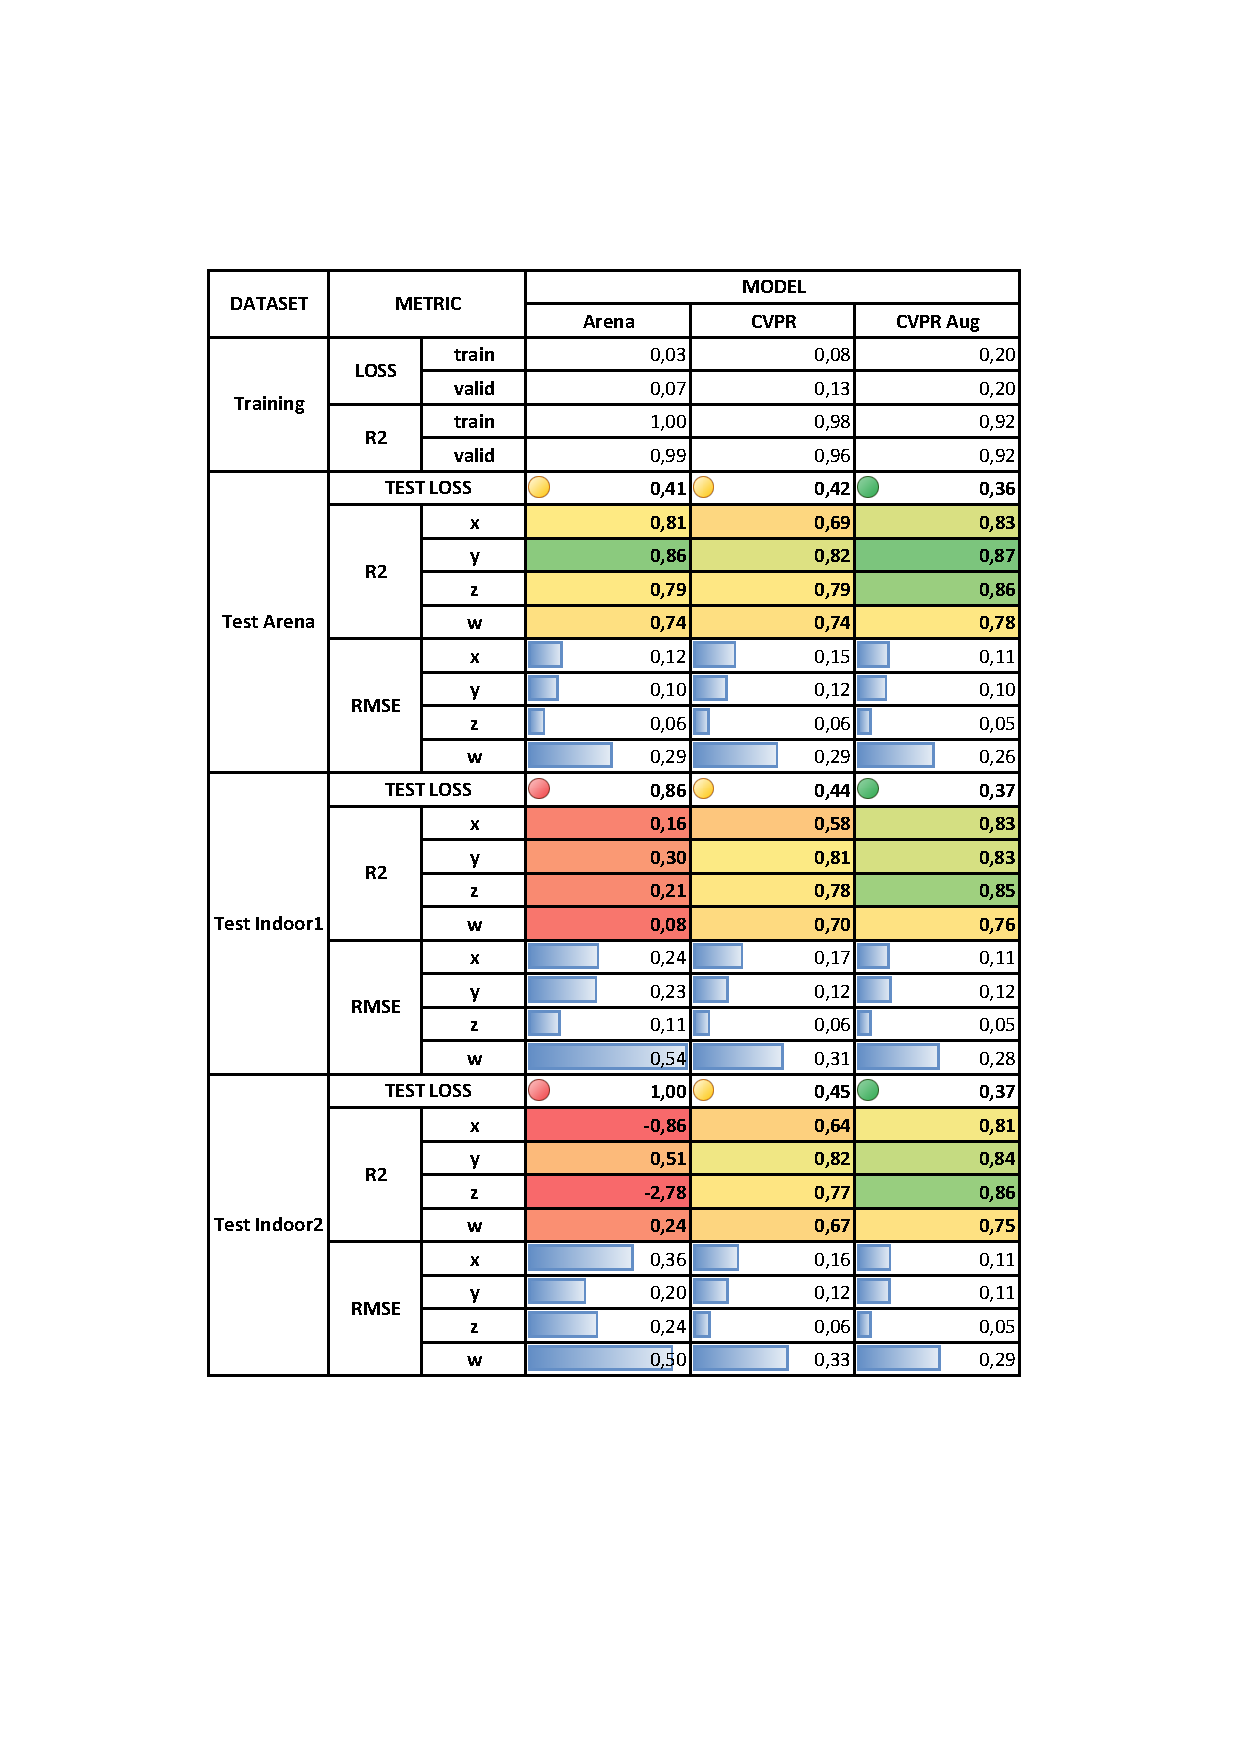
\includepdf[pages={1}, pagecommand={\null\vfill\captionof{table}{Quantitative evaluation: \texttt{Arena}, \texttt{CVPR}, \texttt{CVPR Aug} models on \texttt{arena}, \texttt{indoor1}, \texttt{indoor2} test sets.}\label{tab:qt-summary}}]{contents/images/06-qt-summary}



\section{Qualitative Evaluation}
\label{sec:evaluation-qualitative}

In this section, we do not consider precise metrics for assessing the model's fitness. Instead, we extend the reasoning over numbers and rely on simulations to create various visualizations. These are used to produce a behavioral evaluation of the results. In practice, we confront the models' predictions with the ground truth from a qualitative point of view.

A first evaluation, detailed in Section \ref{subsec:ql-timeline}, presents a comparison with timeline charts. They investigate the general trend of each model on different test sets. Next, in Section \ref{subsec:ql-interactive}, we make use of interactive visualizations to interpret the models' results from a human perspective.



\subsection{Timeline Analysis}
\label{subsec:ql-timeline}

In this section we carefully analyze our three models' behavior on different test sets. This is done through a simulation of about 19 seconds\footnote{the dataset is considered to be collected at 30 \gls{fps}} for comparing the ground truth and the values predicted by each considered model.

For the evaluation, we take into consideration the three test sets presented in the previous section (\texttt{arena}, \texttt{indoor1} and \texttt{indoor2}). Moreover, we add another test set created again through background replacement, as the other two. The difference is that this new test set is composed of a set of multiple backgrounds, rather than a single one. Thus, we call it the \texttt{mixed} test set, composed of a total of 27 backgrounds, which include the 2 indoor scenes of before (Figure \ref{fig:test-indoor}), 3 pictures from the drone arena, 5 textures, and 17 outdoor photos coming from diverse scenarios. Most of the backgrounds in the \texttt{mixed} test set (some are shown in Figure \ref{fig:ql-mixedset}) represent real-world scenes. Hence, we expect them to be particularly challenging for the \texttt{Arena} model. Note that consecutive images in the dataset are randomly assigned to one of the available backgrounds, hence there is no relation between a certain part of the test set and its background.

\begin{figure}[!h]
	\begin{center}
		\begin{subfigure}[h]{0.24\textwidth}
			\centering
			\includegraphics[width=1\textwidth]{"contents/images/06-img-desert"}
		\end{subfigure}
		\hfill
		\begin{subfigure}[h]{0.24\textwidth}
			\centering
			\includegraphics[width=1\textwidth]{"contents/images/06-img-street"}
		\end{subfigure}
		\hfill
		\begin{subfigure}[h]{0.24\textwidth}
			\centering
			\includegraphics[width=1\textwidth]{"contents/images/06-img-beach"}
		\end{subfigure}
		\hfill
		\begin{subfigure}[h]{0.24\textwidth}
			\centering
			\includegraphics[width=1\textwidth]{"contents/images/06-img-park"}
		\end{subfigure}
	\end{center}
	\vspace{-0.5cm}
	\caption[Examples of backgrounds from the \texttt{mixed} test set]{Examples of backgrounds from the \texttt{mixed} test set}
	\label{fig:ql-mixedset}
\end{figure}

\paragraph*{Test set \texttt{arena} (Figure \ref{fig:ql-gtpred-arena})}

All the models achieve good results on the original test set. As in quantitative evaluation, there is no significant difference between the three models. For all variables, the predictions follow the \gls{gt} reasonably accurately. It sometimes happen that one of the models registers slightly better results than the others, but this is a non-systematic behavior. Performance is very similar to the ones presented in Figure \ref{fig:frontalnet-gt-pred}, obtained by the original FrontalNet model according to Mantegazza et al. \cite{mantegazza2019visionbased}.

\begin{figure}[!h]
	\centering
	\includegraphics[width=1 \textwidth]{"contents/images/06-gtpred-arena"}
	\caption[Qualitative evaluation: \gls{gt} vs. predictions results on the \texttt{arena} test set]{Qualitative evaluation: \gls{gt} vs. predictions results on the \texttt{arena} test set}
	\label{fig:ql-gtpred-arena}
\end{figure}


\paragraph*{Test sets \texttt{indoor1} and \texttt{indoor2} (Figures \ref{fig:ql-gtpred-indoor1} and \ref{fig:ql-gtpred-indoor2})}

With artificial test sets, things start to change. None of the networks already know the respective backgrounds\footnote{which means that the three models have not been trained on these new backgrounds}, but severe differences arise between the models. 

\texttt{CVPR} and \texttt{CVPR Aug} are both able to produce predictions very similar to the \gls{gt}, for all the variables. Overall, the model trained on augmented images (the red one in the graphs) appears to be more robust than the other.

On the contrary, the \texttt{Arena} model only follows the ground truth during a tiny percentage of the time, and only for the variables \texttt{Y} and \texttt{W}. Instead, predictions produced for the \texttt{X} and the \texttt{Z} variables seem always irrelevant and totally uncorrelated with the desired value. For \texttt{indoor2}, the variable \texttt{Z} even assumes a value higher than 0.15 for the majority of the time.

\begin{figure}[!h]
	\centering
	\includegraphics[width=1 \textwidth]{"contents/images/06-gtpred-indoor1"}
	\caption[Qualitative evaluation: \gls{gt} vs. predictions results on the \texttt{indoor1} test set]{Qualitative evaluation: \gls{gt} vs. predictions results on the \texttt{indoor1} test set}
	\label{fig:ql-gtpred-indoor1}
\end{figure}

\begin{figure}[H]
	\centering
	\includegraphics[width=1 \textwidth]{"contents/images/06-gtpred-indoor2"}
	\caption[Qualitative evaluation: \gls{gt} vs. predictions results on the \texttt{indoor2} test set]{Qualitative evaluation: \gls{gt} vs. predictions results on the \texttt{indoor2} test set}
	\label{fig:ql-gtpred-indoor2}
\end{figure}


\paragraph*{Test set \texttt{mixed} (Figure \ref{fig:ql-gtpred-mixed})}

Evaluation on the \texttt{mixed} test set further provides evidence that the \texttt{Arena} model is not properly able to predict the user's pose in an unseen scenario. Even worse than before, here the model predictions seem random since they continuously go up and down arbitrarily. This effect, not observed for previous test sets, is due to the composition of the dataset. The \texttt{mixed} test set has different backgrounds for subsequent samples. Thus, the oscillations occur as a symptom of the model sensitivity to the background, as demonstrated through Grad-CAM in Section \ref{sec:model-interpretration}.

Conversely, the models trained on background-replaced training sets can perform their task as they did on the original test set, reasonably following the \gls{gt}.

\begin{figure}[H]
	\centering
	\includegraphics[width=1 \textwidth]{"contents/images/06-gtpred-mixed"}
	\caption[Qualitative evaluation: \gls{gt} vs. predictions results on the \texttt{mixed} test set]{Qualitative evaluation: \gls{gt} vs. predictions results on the \texttt{mixed} test set}
	\label{fig:ql-gtpred-mixed}
\end{figure}


\subsubsection*{Additional analysis on predictions variance}

According to the previous charts, the \texttt{CVPR} and the \texttt{CVPR Aug} models should be able to predict the user's pose in unknown environments. However, the predictions present much more oscillations than the ground truth, even on the \texttt{arena} test set. This phenomenon can lead to undesired consequences when using the model to control the real drone. Strong oscillation can cause the controller to produce unfeasible movements. For this reason, we want to ensure that the variance of our predictions is not much greater than the variance of the ground truth.

\bigskip

We consider different time windows for computing the variance. Each of them bring to the same conclusion. For simplicity, in this thesis we focus on a four seconds window, meaning that we compute the variance every 120 frames. The visualization is done through a timeline, shown in Figure \ref{fig:ql-variance} for the \texttt{arena} and the \texttt{mixed} test sets. From the charts, we observe that the variances over time of both \texttt{CVPR} and \texttt{CVPR Aug} are aligned with the variance of the \gls{gt}. For this reason, we conclude that such models can most likely be used to control the real drone.

\begin{figure}[!h]
	\begin{center}
		\begin{subfigure}[h]{0.49\textwidth}
			\centering
			\includegraphics[width=1\textwidth]{"contents/images/06-variance-arena"}
		\end{subfigure}
		\hfill
		\begin{subfigure}[h]{0.49\textwidth}
			\centering
			\includegraphics[width=1\textwidth]{"contents/images/06-variance-mixed"}
		\end{subfigure}
	\end{center}
	\vspace{-0.5cm}
	\caption[Qualitative evaluation: variance on \texttt{arena} and \texttt{mixed} tests set with a 4 seconds time window]{Qualitative evaluation: variance on \texttt{arena} and \texttt{mixed} tests set with a 4 seconds time window}
	\label{fig:ql-variance}
\end{figure}



\subsection{Per-frame Analysis}
\label{subsec:ql-interactive}

To complete the evaluation, we test the model on new images. Being not able to experiment with a \gls{mocap} system in an unknown environment, we collect new data without having the corresponding ground truth. For this reason, the following assessment is only based on human interpretation.

For simulating the drone's camera, we use a low/medium-tier smartphone from 2017. The device is equipped with a 12 \gls{mp} f/2.2 camera, able to shot 1080p videos at 30 \gls{fps}. Data have been acquired with three different subjects in a large variety of situations, both indoor and outdoor.

We rely on a visualization that simultaneously shows the considered frame and all the necessary information about the variables' predictions. The camera image is in the center, surrounded by the predicted values. Models \texttt{Arena}, \texttt{CVPR}, \texttt{CVPR Aug} are shown with markers in green, blue, and red, respectively. For the analysis, we evaluate the markers' position over the variables axis to check whether they comply with the image. A summary of the variables' interpretation is shown below.

\begin{itemize}
    \item \texttt{X}, on the left, is the distance from the camera. When the user is 1.5 meters distant, the marker is in the center. If the person is further, the marker goes up; otherwise, it goes down.
    \item \texttt{Y}, on the bottom, represents the horizontal alignment. Usually, the relative marker exactly maps the user's position in the image over the x-axis. In other words, when the prediction is correct, the \texttt{Y} marker is precisely under the person in the frame.
    \item \texttt{Z}, on the right, represents the vertical alignment. When the user's face is vertically aligned with the camera, the marker is centered.
    %\footnote{Accordingly, the user's head is visible in the image at a height which is about the 75\% of the y-axis (from the bottom).}.
    If the user lowers, the mark goes down; otherwise, it goes up.
    \item \texttt{W}, on the top, is the orientation of the head. When the user is perfectly facing the camera, the marker will be centered; otherwise, it will follow the user's sight. For example, if the person turns the head on his right, the marker will go left, following the user's gaze.
\end{itemize}

Figure \ref{fig:ql-sim-intro} presents a complete overview of the models' behavior. The examples show many different scenarios: a park, an empty room, a street, different light conditions, weird user's positions, and even a face partially covered by a medical mask. The \texttt{CVPR Aug} model (in red) overall achieves the best results in tracking the user's pose in the image. Variables \texttt{X}, \texttt{Y} and \texttt{Z} generally follow the user properly, without many estimation errors. The \texttt{W} is more prone to fail on its task.

\medskip

The main differences between the three models are observed for the \texttt{X} and the \texttt{Z} variables, coherently with the metrics reported in Table \ref{tab:qt-summary}. This is especially visible when considering tough situations, such as people jumping (Figure \ref{fig:ql-sim-jump}) or running (Figure \ref{fig:ql-sim-run}). The last case also demonstrate that the \texttt{CVPR Aug} model can surprisingly work with a person who is not actually facing the camera.

Some experiments also consider multiple people in the camera's frame. In such situations, \texttt{CVPR Aug} sometimes correctly tracks the foreground person (figure \ref{fig:ql-sim-double-foreground}) while other times does not explicitly choose one to follow (Figure \ref{fig:ql-sim-double-uncertain}). Variables \texttt{X} and \texttt{Y} are the most suited to be considered in such situations, as easily understandable by humans. Many reasons can be the cause of this problem, and further investigation is still needed. We also notice, from Figure \ref{fig:ql-sim-double-change}, that if multiple people are present in the image and one of them moves out of the scene, then the model instantly gives its attention on the remaining person.

% \paragraph*{Head orientation}
% \label{subsec:ql-issue-w}

The main issue which arises from the qualitative evaluation regards the \texttt{W} variable. A large percentage of wrong predictions are made when the user is at the margins of the image. The variable seems affected by the horizontal position of the person, regardless of the head orientation. If the user is in the leftmost part of the frame, \texttt{W} is most likely predicted as if the user is watching on his left (thus, the marker goes on the right part of the axis). Otherwise, when the person is on the right, the \texttt{W} marker often appears on the left. Figure \ref{fig:ql-sim-w-bias} clearly illustrates this phenomenon, which is also observable in other examples. The problem is probably deriving from a bias in the training data, as also stated in \cite{mantegazza2018thesis}.

\begin{figure}[H]
	\begin{center}
		\begin{subfigure}[h]{0.49\textwidth}
			\centering
			\includegraphics[width=0.98\textwidth]{"contents/images/qualitative-videos/perfect1-square01-5681"}
		\end{subfigure}
		\hfill
		\begin{subfigure}[h]{0.49\textwidth}
			\centering
			\includegraphics[width=0.98\textwidth]{"contents/images/qualitative-videos/perfect1-square01-6422"}
		\end{subfigure}
		\vfill
		\begin{subfigure}[h]{0.49\textwidth}
			\centering
			\includegraphics[width=0.98\textwidth]{"contents/images/qualitative-videos/perfect2-house01-5303"}
		\end{subfigure}
		\hfill
		\begin{subfigure}[h]{0.49\textwidth}
			\centering
			\includegraphics[width=0.98\textwidth]{"contents/images/qualitative-videos/perfect2-house01-5329"}
		\end{subfigure}
		\vfill
		\begin{subfigure}[h]{0.49\textwidth}
			\centering
			\includegraphics[width=0.98\textwidth]{"contents/images/qualitative-videos/perfect3-street01-64"}
		\end{subfigure}
		\hfill
		\begin{subfigure}[h]{0.49\textwidth}
			\centering
			\includegraphics[width=0.98\textwidth]{"contents/images/qualitative-videos/perfect3-street01-657"}
		\end{subfigure}
		\vfill
		\begin{subfigure}[h]{0.49\textwidth}
			\centering
			\includegraphics[width=0.98\textwidth]{"contents/images/qualitative-videos/perfect4-house01-6979"}
		\end{subfigure}
		\hfill
		\begin{subfigure}[h]{0.49\textwidth}
			\centering
			\includegraphics[width=0.98\textwidth]{"contents/images/qualitative-videos/dark-courtyard02-5523"}
		\end{subfigure}
		\vfill
		\begin{subfigure}[h]{0.49\textwidth}
			\centering
			\includegraphics[width=0.98\textwidth]{"contents/images/qualitative-videos/perfect4-square01-3488"}
		\end{subfigure}
		\hfill
		\begin{subfigure}[h]{0.49\textwidth}
			\centering
			\includegraphics[width=0.98\textwidth]{"contents/images/qualitative-videos/perfect5-square02-1252"}
		\end{subfigure}
		\vfill
	\end{center}
	\vspace{-0.5cm}
	\caption[Qualitative evaluation: overview of the models' behavior on newly recorded images]{Qualitative evaluation: overview of the models' behavior on newly recorded images}
	\label{fig:ql-sim-intro}
\end{figure}

\begin{figure}[H]
	\begin{center}
		\begin{subfigure}[h]{0.49\textwidth}
			\centering
			\includegraphics[width=0.98\textwidth]{"contents/images/qualitative-videos/jump1-park01-2943"}
		\end{subfigure}
		\hfill
		\begin{subfigure}[h]{0.49\textwidth}
			\centering
			\includegraphics[width=0.98\textwidth]{"contents/images/qualitative-videos/jump1-park01-3079"}
		\end{subfigure}
		\vfill
		\begin{subfigure}[h]{0.49\textwidth}
			\centering
			\includegraphics[width=0.98\textwidth]{"contents/images/qualitative-videos/jump2-square02-329"}
		\end{subfigure}
		\hfill
		\begin{subfigure}[h]{0.49\textwidth}
			\centering
			\includegraphics[width=0.98\textwidth]{"contents/images/qualitative-videos/jump2-square02-369"}
		\end{subfigure}
	\end{center}
	\vspace{-0.5cm}
	\caption[Qualitative evaluation: models' behavior on jumping people]{Qualitative evaluation: models' behavior on jumping people. The \texttt{Z} variable is correctly predicted only by the \texttt{CVPR Aug} (red) model.}
	\label{fig:ql-sim-jump}
\end{figure}

\begin{figure}[H]
	\begin{center}
		\begin{subfigure}[h]{0.49\textwidth}
			\centering
			\includegraphics[width=0.98\textwidth]{"contents/images/qualitative-videos/running1-square02-712"}
		\end{subfigure}
		\hfill
		\begin{subfigure}[h]{0.49\textwidth}
			\centering
			\includegraphics[width=0.98\textwidth]{"contents/images/qualitative-videos/running1-square02-6969"}
		\end{subfigure}
		\vfill
		\begin{subfigure}[h]{0.49\textwidth}
			\centering
			\includegraphics[width=0.98\textwidth]{"contents/images/qualitative-videos/running1-square02-7278"}
		\end{subfigure}
		\hfill
		\begin{subfigure}[h]{0.49\textwidth}
			\centering
			\includegraphics[width=0.98\textwidth]{"contents/images/qualitative-videos/running1-square02-7323"}
		\end{subfigure}
	\end{center}
	\vspace{-0.5cm}
	\caption[Qualitative evaluation: models' behavior on running people]{Qualitative evaluation: models' behavior on running people. \texttt{CVPR} is even worse than the \texttt{Arena} model. \texttt{CVPR Aug} is mostly superior for the \texttt{X} and the \texttt{W} variables.}
	\label{fig:ql-sim-run}
\end{figure}

\begin{figure}[H]
	\begin{center}
		\begin{subfigure}[h]{0.49\textwidth}
			\centering
			\includegraphics[width=0.98\textwidth]{"contents/images/qualitative-videos/double1-square02-1708"}
		\end{subfigure}
		\hfill
		\begin{subfigure}[h]{0.49\textwidth}
			\centering
			\includegraphics[width=0.98\textwidth]{"contents/images/qualitative-videos/double1-square02-1895"}
		\end{subfigure}
		\vfill
		\begin{subfigure}[h]{0.49\textwidth}
			\centering
			\includegraphics[width=0.98\textwidth]{"contents/images/qualitative-videos/double4-square02-5065"}
		\end{subfigure}
		\hfill
		\begin{subfigure}[h]{0.49\textwidth}
			\centering
			\includegraphics[width=0.98\textwidth]{"contents/images/qualitative-videos/double4-square02-5239"}
		\end{subfigure}
	\end{center}
	\vspace{-0.5cm}
	\caption[Qualitative evaluation: models' behavior on multiple people]{Qualitative evaluation: models' behavior on multiple people. In all the images, the models track the person in the foreground, as desired. Focus on \texttt{X} and \texttt{Y} for briefly understanding what is going on behind the models' reasoning. The reason behind such precision is probably found on the far distance of the background user and even on its clothes color. The most surprising result is observed in the 4th frame, for which the foreground user is detected even if it appears at the bottom of the image.}
	\label{fig:ql-sim-double-foreground}
\end{figure}

\begin{figure}[H]
	\begin{center}
		\begin{subfigure}[h]{0.49\textwidth}
			\centering
			\includegraphics[width=0.98\textwidth]{"contents/images/qualitative-videos/double2-square02-2644"}
		\end{subfigure}
		\hfill
		\begin{subfigure}[h]{0.49\textwidth}
			\centering
			\includegraphics[width=0.98\textwidth]{"contents/images/qualitative-videos/double2-square02-2896"}
		\end{subfigure}
		\vfill
		\begin{subfigure}[h]{0.49\textwidth}
			\centering
			\includegraphics[width=0.98\textwidth]{"contents/images/qualitative-videos/double3-square02-3940"}
		\end{subfigure}
		\hfill
		\begin{subfigure}[h]{0.49\textwidth}
			\centering
			\includegraphics[width=0.98\textwidth]{"contents/images/qualitative-videos/double3-square02-4210"}
		\end{subfigure}
		\vfill
		\begin{subfigure}[h]{0.49\textwidth}
			\centering
			\includegraphics[width=0.98\textwidth]{"contents/images/qualitative-videos/double6-street01-1978"}
		\end{subfigure}
		\hfill
		\begin{subfigure}[h]{0.49\textwidth}
			\centering
			\includegraphics[width=0.98\textwidth]{"contents/images/qualitative-videos/double6-street01-2017"}
		\end{subfigure}
	\end{center}
	\vspace{-0.5cm}
	\caption[Qualitative evaluation: models' behavior on multiple people]{Qualitative evaluation: models' behavior on multiple people. The models is highly uncertain on the person who must track. Focus on \texttt{X} and \texttt{Y} for briefly understanding what is going on behind the models' reasoning. From left to right, top to bottom, the foreground person is tracked in images 1 and 4. In the others, the background person is taking the model attention. This can be due to specific distances, clothes colors, and also faces partially covered by a mask.}
	\label{fig:ql-sim-double-uncertain}
\end{figure}

\begin{figure}[H]
	\begin{center}
		\begin{subfigure}[h]{0.49\textwidth}
			\centering
			\includegraphics[width=0.98\textwidth]{"contents/images/qualitative-videos/double5-square03-1489"}
		\end{subfigure}
		\hfill
		\begin{subfigure}[h]{0.49\textwidth}
			\centering
			\includegraphics[width=0.98\textwidth]{"contents/images/qualitative-videos/double5-square03-1512"}
		\end{subfigure}
	\end{center}
	\vspace{-0.5cm}
	\caption[Qualitative evaluation: models' behavior on multiple people]{Qualitative evaluation: models' behavior on multiple people. As soon as the person in the right moves out, the seated user becomes tracked by the model.}
	\label{fig:ql-sim-double-change}
\end{figure}



\begin{figure}[H]
	\begin{center}
		\begin{subfigure}[h]{0.49\textwidth}
			\centering
			\includegraphics[width=0.98\textwidth]{"contents/images/qualitative-videos/W-bias-house01-2380"}
		\end{subfigure}
		\hfill
		\begin{subfigure}[h]{0.49\textwidth}
			\centering
			\includegraphics[width=0.98\textwidth]{"contents/images/qualitative-videos/W-bias-house01-7019"}
		\end{subfigure}
		\vfill
		\begin{subfigure}[h]{0.49\textwidth}
			\centering
			\includegraphics[width=0.98\textwidth]{"contents/images/qualitative-videos/W-bias-park01-4209"}
		\end{subfigure}
		\hfill
		\begin{subfigure}[h]{0.49\textwidth}
			\centering
			\includegraphics[width=0.98\textwidth]{"contents/images/qualitative-videos/W-bias-park01-7983"}
		\end{subfigure}
		\vfill
		\begin{subfigure}[h]{0.49\textwidth}
			\centering
			\includegraphics[width=0.98\textwidth]{"contents/images/qualitative-videos/W-bias-square01-8090"}
		\end{subfigure}
		\hfill
		\begin{subfigure}[h]{0.49\textwidth}
			\centering
			\includegraphics[width=0.98\textwidth]{"contents/images/qualitative-videos/W-bias-square01-8434"}
		\end{subfigure}
	\end{center}
	\vspace{-0.5cm}
	\caption[Qualitative evaluation: \texttt{CVPR Aug} issue on \texttt{W} variable]{Qualitative evaluation: \texttt{CVPR Aug} issue on \texttt{W} variable. When the user is on one side, most of the time, the \texttt{W} is predicted on the opposite side. Only the last image is showing a correct behavior, which is anyway caused by the same bias that affects the wrong predictions.}
	\label{fig:ql-sim-w-bias}
\end{figure}